\subsection{Section II: Analysis of Performance of Classifiers}
\subsubsection{Classifier Performance for Iris Dataset}
	\textbf{Classifier 1}\\
	\begin{itemize}
		\item Preprocessing - Simple Scaling
		\item Proximity Metric - Euclidean Distance
		\item Voting - Inverse Distance Weighted Voting
	\end{itemize}
	The confusion matrix for three different values of k is given in Fig: ?
	\begin{figure}[h]
			\label{fig:iris_k=1}
			\caption{Confusion Matrix k = 1 (Datset:Iris Classifier:1)}
			\centering
			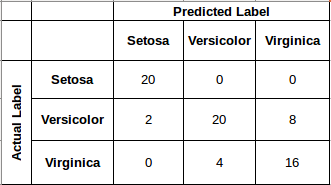
\includegraphics[width=0.3\textwidth]{images/iris_k1.png}
	\end{figure}
	\begin{figure}[h]
		\label{fig:iris_k=5}
		\caption{Confusion Matrix k = 5 (Datset:Iris Classifier:1)}
		\centering
		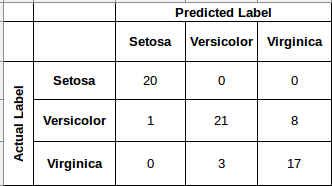
\includegraphics[width=0.3\textwidth]{images/iris_k=5.png}
	\end{figure}
	\begin{figure}[h]
		\label{fig:iris_k=10}
		\caption{Confusion Matrix k = 10 (Datset:Iris Classifier:1)}
		\centering
		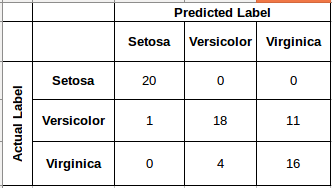
\includegraphics[width=0.3\textwidth]{images/iris_k=10.png}
	\end{figure}	
	??Analysis??\\
	
	\textbf{Classifier 2}\\
	\begin{itemize}
		\item Preprocessing - Simple Scaling (same as before)
		\item Proximity Metric - Cosine Similarity
		\item Voting - Inverse Distance Weighted Voting (same as before)
	\end{itemize}
	The confusion matrix is given in Fig: ??(use excel)
	\begin{figure}[h]
			\label{fig:iris_cosine_k=1}
			\caption{Confusion Matrix k = 1 (Datset:Iris Classifier:2)}
			\centering
			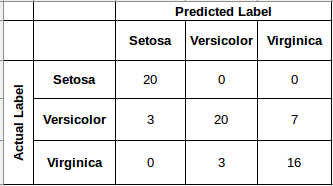
\includegraphics[width=0.3\textwidth]{images/iris_cosine_k=1.png}
	\end{figure}
	\begin{figure}[h]
		\label{fig:iris_consine_k=5}
		\caption{Confusion Matrix k = 5 (Datset:Iris Classifier:2)}
		\centering
		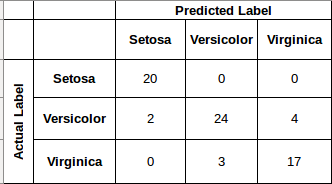
\includegraphics[width=0.3\textwidth]{images/iris_cosine_k=5.png}
	\end{figure}
	\begin{figure}[h]
		\label{fig:iris_cosine_k=10}
		\caption{Confusion Matrix k = 10 (Datset:Iris Classifier:2)}
		\centering
		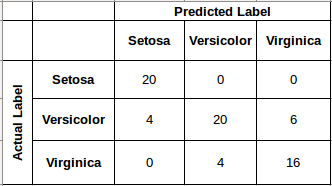
\includegraphics[width=0.3\textwidth]{images/iris_cosine_k=10.png}
	\end{figure}
	??Analysis??

\subsubsection{Classifier Performance for Income Dataset}
To analyze the performance of kNN on the Income dataset two parameters need to be determined. The number of nearest neighbours $k$ and threshold for making the prediction. To optimum $k$ for the classifier would be the $k$ for which the ``Area Under the Roc Curve" is maximized. To do this, the roc graphs were computed over the test set for $k$'s ranging from 1 to 100. The Area under the curve increases as k increase. This means that the classifer is getting better at all levels. However after a while it peaks and then plateus. The $k$ at the peak can be chosen as of the best $k$'s.

\textbf{Classifier 1}\\
	\begin{itemize}
		\item Preprocessing - Simple Scaling
		\item Proximity Metric - Euclidean Distance
		\item Voting - Inverse Distance Weighted Voting
	\end{itemize}
	The confusion matrix is given in Fig: ??(use excel)\\
	The ROC curve is given in Fig: ??\\
	For this classifier the Area under ROC reaches maximum at k = 38 \\
	\begin{figure}[h]
		\label{fig:classifier1_auc}
		\caption{Plot of Area Under the Roc curve for different values of k for Income Classifier 1. Maxima is achieved at k = 36}
		\centering
		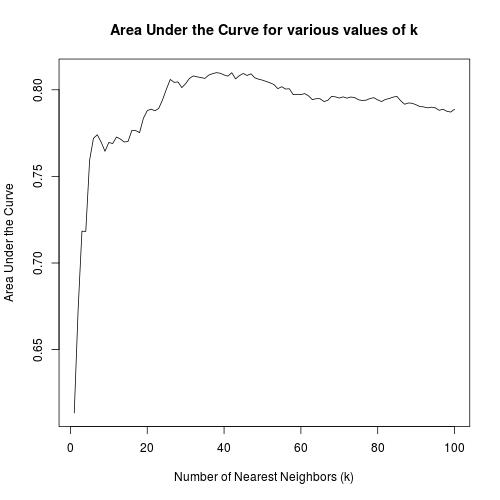
\includegraphics[width=0.3\textwidth]{images/income_classifier1/auc.jpg}
	\end{figure}	
	\begin{figure}
		\label{fig:classifier1_roc}
		\caption{ROC curves for different values of k for Income Classifier 1}
		\centering
		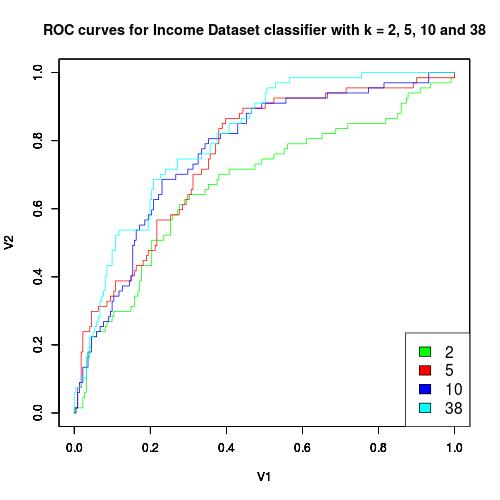
\includegraphics[width=0.3\textwidth]{images/income_classifier1/roc.jpg}
	\end{figure}
	\begin{figure}
		\label{fig:classifier1_accuracy}
		\caption{Plot of Accuracy Vs Threshold Values for k = 38}
		\centering
		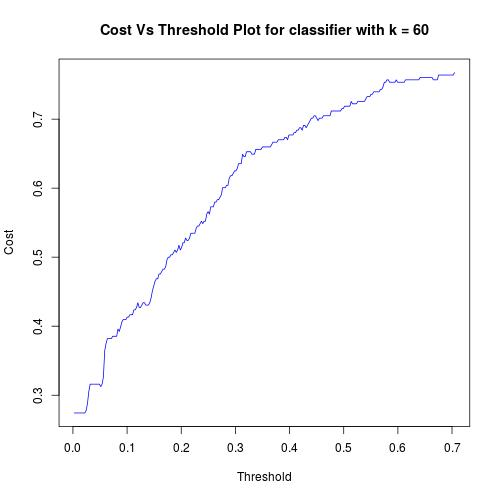
\includegraphics[width=0.3\textwidth]{images/income_classifier1/accuracy.jpg}
	\end{figure}	
	
\textbf{Classifier 2}\\
	\begin{itemize}
		\item Preprocessing - Simple Scaling
		\item Proximity Metric - Cosine Similarity
		\item Voting - Inverse Distance Weighted Voting
	\end{itemize}
	The confusion matrix is given in Fig: ??(use excel)\\
	The ROC curve is given in Fig: ??\\
	Max for k = 36??Analysis??\\
	\begin{figure}[h]
		\label{fig:classifier2_auc}
		\caption{Plot of Area Under the Roc curve for different values of k for Income Classifier 2. Maxima is achieved at k = 36}
		\centering
		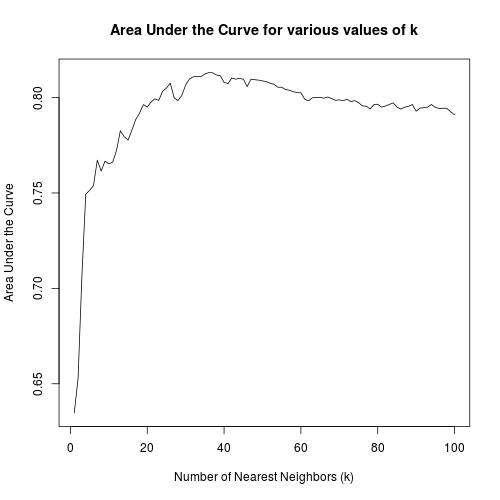
\includegraphics[width=0.3\textwidth]{images/income_classifier2/auc.jpg}
	\end{figure}	
	\begin{figure}
		\label{fig:classifier2_roc}
		\caption{ROC curves for different values of k for Income Classifier 2}
		\centering
		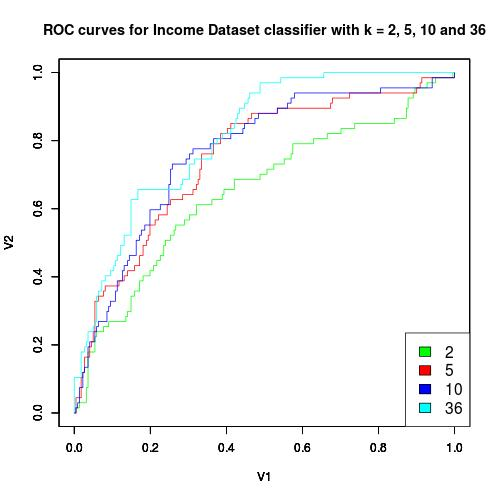
\includegraphics[width=0.3\textwidth]{images/income_classifier2/roc.jpg}
	\end{figure}
	\begin{figure}
		\label{fig:classifier2_accuracy}
		\caption{Plot of Accuracy Vs Threshold Values for k = 36}
		\centering
		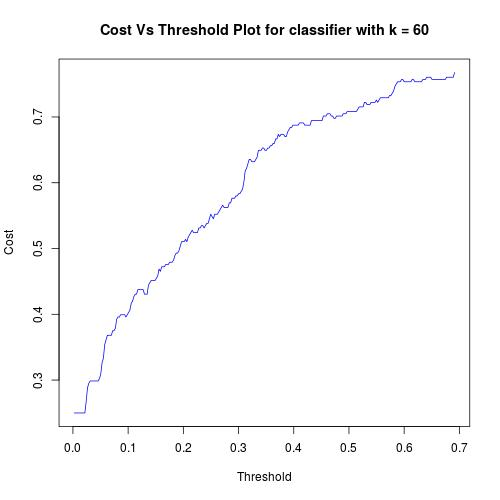
\includegraphics[width=0.3\textwidth]{images/income_classifier2/accuracy.jpg}
	\end{figure}
	
\textbf{Classifier 3} - Best Performance\\
	\begin{itemize}
		\item Preprocessing - Simple Scaling with Binning
		\item Proximity Metric - 
		\item Voting - Inverse Distance Weighted Voting with Positive Class Priority
	\end{itemize}
	The confusion matrix is given in Fig: ??(use excel)\\
	The ROC curve is given in Fig: ??\\
	??Analysis??\\
	\begin{figure}[h]
		\label{fig:classifier3_auc}
		\caption{Plot of Area Under the Roc curve for different values of k for Income Classifier 3. Accuracy keeps getting beyond hundred}
		\centering
		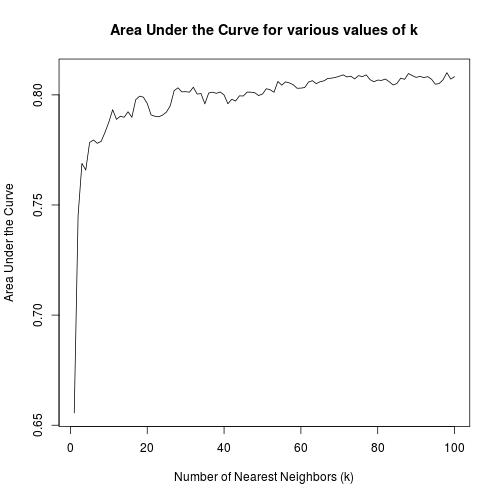
\includegraphics[width=0.3\textwidth]{images/income_classifier3/auc.jpg}
	\end{figure}	
	\begin{figure}
		\label{fig:classifier1_roc}
		\caption{ROC curves for different values of k for Income Classifier 3}
		\centering
		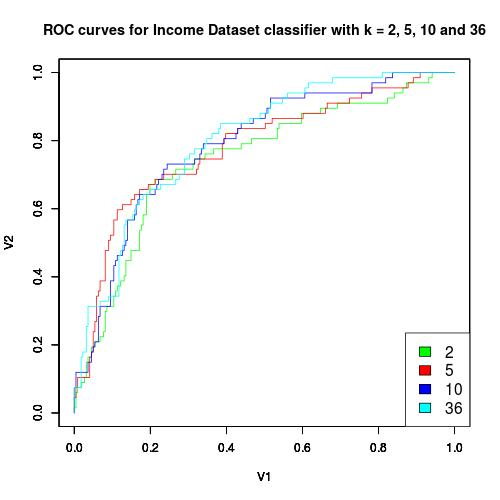
\includegraphics[width=0.3\textwidth]{images/income_classifier3/roc.jpg}
	\end{figure}
	\begin{figure}
		\label{fig:classifier3_accuracy}
		\caption{Plot of Accuracy Vs Threshold Values for k = 40}
		\centering
		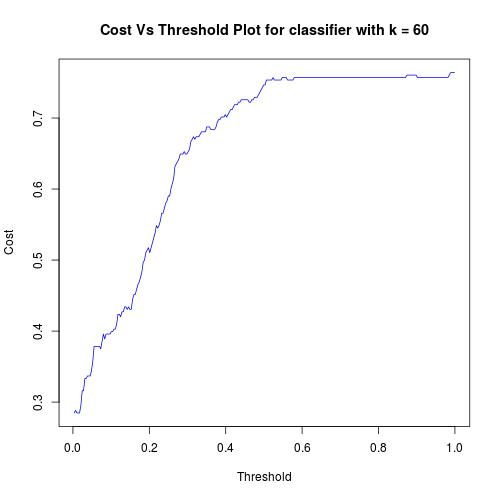
\includegraphics[width=0.3\textwidth]{images/income_classifier3/accuracy.jpg}
	\end{figure}
